\def\year{2016}\relax
%File: formatting-instruction.tex
\documentclass[letterpaper]{article}
\usepackage{aaai16}
\usepackage{times}
\usepackage{helvet}
\usepackage{courier}

\usepackage{graphicx}
\usepackage{fullpage}
\usepackage[hidelinks]{hyperref}
\usepackage{amsfonts}
\usepackage{amsmath}
\usepackage{amssymb}
\usepackage{amsthm}
\usepackage{bbm}
\usepackage{natbib}
\usepackage{clrscode3e}
\usepackage{tcolorbox}

% Basic mathematical notation
\newcommand{\R}{\mathbb{R}}
\newcommand{\E}{\mathbb{E}}
\newcommand{\expct}[1]{\E\left[#1\right]}
\renewcommand{\P}{\mathbb{P}}
\newcommand{\one}{\mathbb{I}}
\newcommand{\mat}[1]{\mathbf{#1}}
%\newcommand{\dim}{\operatorname{dim}}
\newcommand{\rank}{\operatorname{rank}}
\newcommand{\diag}{\operatorname{diag}}
\newcommand{\vecm}{\operatorname{vec}}
\newcommand{\dist}{\mathsf{dist}}
\newcommand{\norm}[1]{\|#1\|}
\newcommand{\sval}{\mathfrak{s}}

% Names of norms and vector spaces
\newcommand{\ltwo}{\ell^2}
\newcommand{\lone}{\ell^1}
\newcommand{\lp}{\ell^p}
\newcommand{\lpq}{\ell^q}
\newcommand{\ltworat}{\ell^2_{\cR}}
\newcommand{\lonerat}{\ell^1_{\cR}}
\newcommand{\lprat}{\ell^p_{\cR}}
\newcommand{\inner}[2]{\langle #1, #2 \rangle}

% Notation for MPD and POMDP
\newcommand{\mdp}{\langle S, A, T, r, d_0\rangle}
\newcommand{\pomdp}{\langle S, A, T, r, \Omega, O, \bzero \rangle}
% Notation for weighted automata
\newcommand{\sstar}{\Sigma^\star}
\newcommand{\cF}{\mathcal{F}}
\newcommand{\cR}{\mathcal{R}}
\newcommand{\A}{\mat{A}}
\newcommand{\B}{\mat{B}}
\newcommand{\ahist}{\boldsymbol{\alpha}_h}
\newcommand{\bhist}{\boldsymbol{\beta}_h}
\newcommand{\azero}{\boldsymbol{\alpha}_0}
\newcommand{\tazero}{\tilde{\boldsymbol{\alpha}}_0}
\newcommand{\hazero}{\hat{\boldsymbol{\alpha}}_0}
\newcommand{\ainf}{\boldsymbol{\alpha}_{\infty}}
\newcommand{\hainf}{\hat{\boldsymbol{\alpha}}_{\infty}}
\newcommand{\tainf}{\tilde{\boldsymbol{\alpha}}_{\infty}}
\newcommand{\bzero}{\boldsymbol{\beta}_0}
\newcommand{\binf}{\boldsymbol{\beta}_{\infty}}
\newcommand{\wa}{\langle \azero, \ainf, \{\A_\sigma\} \rangle}
\newcommand{\wA}{\langle \azero, \{\A_\sigma\} \rangle}
\newcommand{\waS}{\langle \azero, \ainf, \{\A_\sigma\}_{\sigma \in \Sigma} \rangle}
\newcommand{\wbS}{\langle \bzero, \binf, \{\B_\sigma\}_{\sigma \in \Sigma} \rangle}
\newcommand{\waQ}{\langle \mQ^\top \azero, \mQ^{-1} \ainf, \{\mQ^{-1} \A_\sigma
\mQ\} \rangle}
\newcommand{\hwa}{\langle \hazero, \hainf, \{\hat{\A}_\sigma\} \rangle}
\newcommand{\twa}{\langle \tazero, \tainf, \{\tilde{\A}_\sigma\} \rangle}
\newcommand{\wb}{\langle \bzero, \binf, \{\B_\sigma\} \rangle}
\newcommand{\waV}{\langle \azero, \phi, \{\tau_\sigma\} \rangle}
\newcommand{\wasigma}{\langle \azero, \ainf, \{\A_\sigma\}_{\sigma \in \Sigma} \rangle}
\newcommand{\alamb}{\boldsymbol{\alpha}_{\lambda}}
\newcommand{\ainfa}{\boldsymbol{\alpha}_{a}}
\newcommand{\wapS}{\langle \alamb, \{\ainfa\}_{a \in A}, \{\A_\sigma\}_{\sigma \in \Sigma} \rangle}
\newcommand{\wap}{\langle \alamb, \{\ainfa\}, \{\A_\sigma\} \rangle}
\newcommand{\wAp}{\langle \alamb, \{\A_\sigma\} \rangle}

% Sets with name
\newcommand{\Ps}{\mathcal{P}}
\newcommand{\Ss}{\mathcal{S}}
\newcommand{\cD}{\mathcal{D}}
\newcommand{\cA}{\mathcal{A}}
\newcommand{\cB}{\mathcal{B}}

% Special norms
\newcommand{\normop}[1]{\|#1\|_{\mathrm{op}}}
\newcommand{\normhk}[1]{\|#1\|_{\mathrm{hk}}}

% (Blocks of) Hankel matrices
\renewcommand{\H}{\mat{H}}
\newcommand{\hr}{\mat{h}_{\lambda,\Ss}}
\newcommand{\hc}{\mat{h}_{\Ps,\lambda}}

% Named matrices and vectors
\renewcommand{\v}{\mat{v}}
\newcommand{\mM}{\mat{M}}
\newcommand{\mP}{\mat{P}}
\newcommand{\mS}{\mat{S}}
\newcommand{\mG}{\mat{G}}
\newcommand{\mU}{\mat{U}}
\newcommand{\mV}{\mat{V}}
\newcommand{\mD}{\mat{D}}
\newcommand{\mQ}{\mat{Q}}
\newcommand{\mI}{\mat{I}}
\newcommand{\mT}{\mat{T}}
\renewcommand{\mp}{\mat{p}}
\newcommand{\me}{\mat{e}}

% Environments for mathematical statements
\newtheorem{theorem}{Theorem}
\newtheorem{proposition}[theorem]{Proposition}
\newtheorem{lemma}[theorem]{Lemma}
\newtheorem{corollary}[theorem]{Corollary}
\newtheorem{example}[theorem]{Example}
\newtheorem{problem}[theorem]{Problem}
\newtheorem{definition}[theorem]{Definition}
%\newtheorem{conjecture}[theorem]{Conjecture}
\theoremstyle{remark}
\newtheorem{remark}{Remark}

% added by e2crawfo
\DeclareMathOperator*{\argmin}{arg\,min}
\DeclareMathOperator*{\argmax}{arg\,max}

\newcommand{\be}{b}
\newcommand{\jcost}[1]{\sum_{t=1}^T E_{s \sim d^t_{#1}}[C_{#1}(s)]}
\newcommand{\lloss}[4]{E_{#1 \sim d_{#3}, a \sim \pi^*(#1)}[\ell(#2, a, #4)]}
\newcommand{\exprt}[1]{\pi^*(#1)}
\newcommand{\pihat}[1]{\hat{\pi}_{#1}}
\newcommand{\hinge}[1]{\left[1 - #1\right]_+}

\newcommand\independent{\protect\mathpalette{\protect\independenT}{\perp}}
\def\independenT#1#2{\mathrel{\rlap{$#1#2$}\mkern2mu{#1#2}}}


\newcommand{\fg}{Fig.}
\newcommand{\eg}{e.g. }
\newcommand{\ie}{i.e. }
\frenchspacing
\setlength{\pdfpagewidth}{8.5in}
\setlength{\pdfpageheight}{11in}
\pdfinfo{
/Title (Learning Multiple Mixtures of Sequence Generators)
/Author (Eric Crawford, Joelle Pineau)}
\setcounter{secnumdepth}{0}
 \begin{document}
% The file aaai.sty is the style file for AAAI Press 
% proceedings, working notes, and technical reports.
%
\title{Multitask and Transfer Learning via Mixtures of Shared Sequence Generators}
\author{Eric Crawford, Joelle Pineau\\
Reasoning and Learning Lab, McGill University\\
}
\maketitle
\begin{abstract}
    Multitask learning explores techniques for learning in situations wherein one is confronted with several tasks simultaneously. In such cases, it is often possible to improve performance on all tasks by sharing information, and having the learning of each task be influenced by data from all tasks. This is particularly true when there are many tasks each with a small amount of data. Thus far, the majority of work in this field has targeted the classification and regression settings, while comparatively little work has looked at multitask learning for sequential data. In this article we work towards filling this void. In particular, we identify a common form of relatedness between sequence learning tasks, wherein the sequence-generating system underlying each task is a probabilistic mixture of several more elementary sequence-generating systems, with the elementary systems shared between tasks. We then present a Bayesian algorithm capable of exploiting this form of task relatedness. We report experiments on both synthetic and real data, showing that our algorithm successfully shares data between tasks, achieving improved performance compared to all baseline algorithms. The algorithm is shown to be capable of handling sequences composed of either discrete or continuous observations, and to be capable of accommodating different assumptions with regard to the form of the elementary sequence generators.

    % multiple which seek to improve performance when multiple, related tasks are studies learning algorithms that take advantage of data from multiple, related tasks in order to improve generalization performance on all tasks. One way to think of this is inductive bias: we make some assumption on how the tasks are related to one another, which informs our learning algorithm, narrowing-down the set of meta-hypotheses that we consider, which has the effect of lowering sample complexity as long the inductive assumption is satisfied. The literature on multitask learning for classification and regression is large and mature, while comparatively little work has been done on multitask approaches for sequence learning. Here we seek to fill this void, identifying a collection of important multitask sequence learning problems, and provide an algorithm for solving them based on Latent Dirichlet Allocation, a Bayesian learning algorithm originally developed for modelling collections of natural language documents.
\end{abstract}

\noindent

Multitask learning seeks to improve performance on multiple related learning tasks by learning the tasks simultaneously and sharing information between them. A central notion for machine learning, though especially for multitask learning, is that of \textit{inductive bias}. Inductive bias captures the collection of assumptions that are made, either explicitly or implicitly, about the nature of the world when applying a learning algorithm to obtain a hypothesis from training data. Importantly, inductive bias is the reason that generalization is possible at all; without making such assumptions (and having them be true), it is impossible for data generated from a system to be informative about what kind of data might be generated from that system in the future.

A common example of an inductive bias in regression settings is that the function to be learned is smooth. This assumption gives us power, since when we are trying to learn a function from a collection of data, it allows us to rule out those functions which would not be smooth on the training data set. If we throw this assumption away, then we obtain no generalization power from the training data, since the values of the function at input points other than those seen during training are completely unconstrained by the training data points.

In multitask learning, inductive bias plays a role at two separate levels. First, it has the role that is plays in all machine learning, influencing the manner in which training data from each task affects our selection of a hypothesis for that task. Second, it plays a role at a higher level of abstraction, influencing the way in which data from each task affects our selection of hypotheses for \textit{other} tasks.

Coming up with new mechanisms for sharing data between tasks, then, generally consists of coming up with new forms of inductive bias, at this second level of abstraction, that will be commonly encountered in real data.

One mechanism for sharing information between tasks that has been successfully applied to both classification and regression problems consists of assuming that the true hypothesis for each task can be expressed as a sparse linear combination of a shared collection of basis vectors. We can think of the shared basis vectors as a common ``dictionary'' of vectors, and so algorithms that make use of this approach are often called dictionary learning algorithms. One instance of this idea is Grouping and Overlap Multitask Learning (GO-MTL) \citep{kumar2012learning}, which can be applied when learning collections of linear hypotheses, and yields improved performance when there are groups of similar tasks or tasks whose hypothese ``overlap''. They provide an objective function and an accompanying optimization algorithm which effectively identifies groups of common tasks and, for each group, uses data from all tasks in the group to improve the learning of the hypothesis that the group shares. See also \citet{zhang2008flexible} which aims to provide a more general formulation of this overall idea.
TODO: This paper actually covers a framework wherein the PARAMETERS are linear combinations of a basis. Are we making the same assumption? Not quite. If we transferred that over to the sequence learning case, we would get something more in line with the Simplicial mixtures of markov chains.
%(i.e. there are a small number of groups of tasks, and all tasks within a group use the same linear function),

An alternative to regression or classification is \textit{sequence learning}. In single task sequence learning, we are given, as training data, a collection of sequences of observations generated by some system. The learning task is to identify a function which, given the beginning of a sequence generated from the same system, is capable of predicting the next observation or the remainder of the sequence. In multitask sequence learning, we are given training sequences generated by several different systems, and at test time, given the start of a sequence as well as an indication of which system it was generated from, predict the remainder of the sequence. If the systems are related in some way, then we can hope to use data from all the systems to improve our overall performance.

The current work extends the dictionary learning idea to the sequence learning setting, providing a novel mechanism for sharing information between sequence learning tasks. In particular, we assume that the system generating sequences for each task is actually a mixture of a smaller dictionary of elementary systems. This turns out to be equivalent to assuming that each task's probability distribution over sequences is a convex combination of a dictionary of basis probability distributions, further echoing the dictionary learning assumptions. We propose a Bayesian algorithm for exploiting such collections of tasks which is closely related to Latent Dirichlet Allocation (a technique for extracting topics from collections of natural language documents).

% This mechanism shares some of the intuition from GO-MTL in that it assumes that the hypthothesis for each task is a sparse linear combination of a core dictionary of hypotheses whose size is smaller than the number of tasks. The difference is that here our hypotheses and dictionary elements are distributions over strings, whereas in GO-MTL they are linear functions.

% Need to tease apart generalization (performance on unseen points) from performance on points we have seen before, but which might take on different values in the future because of randomness. This latter point is important for inductive bias as it applies to multitask learning, since, unless we do transfer learning, we're going to be tested on ``points'' (tasks) that we have seen before. Think we can probably still cast it as generalization, but need a slightly more nuanced definition of generalization.
% 
% We are attempting to predict a distribution for each task. Similar to any kind of regression with output noise; the output value for any input value (task index) is a random variable whose distribution we want to learn. 
% 
% Multitask learning makes use of inductive bias at a slightly higher level of abstraction than typical machine learning.
% 
% As a general rule, it is crucial that the inductive bias assumption be \textit{correct} (that is, actually apply to the data one is working with), otherwise this assumption/information will not influence the hypothesis search process in the correct way.
% 
% However, in some cases where the inductive bias assumption is incorrect, making the assumption can still improve performance by acting as a regularizer. Because we have little data, the hypothesis chosen in the regularized space, even if said space does not contain the true hypothesis, may perform better than the hypothesis chosen in the (much larger) unregularized space.
% 
% Again this difference between regularization and simple side information. Maybe a good way to summarize regularization: an assumption that is made because we can't even hope to do well without it, because we have so little data. In linear regression, if the amount of data is very small, then there is no way we are going to be able to estimate the correct regression co-efficients if we leave the range unconstrained. So we have to constrain the norm of the coefficients. But what if the coefficients actually do have large norm? Well then we couldn't have hoped to do well anyway; and maybe there is some sense in which forcing the coefficients to be small somehow reduces the size of the errors that you make, when you make them. In the case of linear regression, it puts a limit on the slope of plane. So kind of a smoothness assumption; I feel like there must be something to this, otherwise why not pick any other arbitrary ball, and confine our hypotheses to that. Its like saying we don't have enough information to nail down the high-frequency components, so we're going to settle for the low frequency components.
% 
% Tease apart assumption vs information. Kind of like the distinction between belief and knowledge (justified true belief). By calling something information, we are asserting that is true.
% 
% To obtain improved performance in a multitask learning setting (compared to the baselines of either learning each task indvidually), one generally needs to make an assumption about how the tasks are related. 
% 
% * Inductive Bias
% * Improving performance on all tasks.
% * Having information from tasks inform the learning of other tasks.
% * The interaction of these two ideas; inductive bias, and information flowing to other tasks.
% * Lack of work on sequence learning.

\section{Multitask Sequence Learning}
Multitask sequence learning can be formalized as follows. Assume we are given $T$ sequence prediction tasks. The training data for each task consists of a collection of $N$ sequences. From this training data we wish to select a collection of hypotheses (or a single ``meta''-hypothesis) $\{H_t\}_{t=1}^T$ which will provide the most accurate predictions on a test dataset containing data from each task.

\subsection{Mixtures of Shared Sequence Generators}
When transplanting LDA to the sequence learning setting, one obtains a model which we call \textbf{SequentialLDA}.
* We have a set of elementary sequence generators, $G^{(i)}(x_1\dots x_n)$, where $G^{(i)}(\dot)$ is a probability distribution over strings. Each task is a convex combination (or mixture) $\theta^{(t)}$ of these elementary generators. To generate a sequence for task $t$, we first select an elementary generator according to $\theta^{(t)}$ (selecting $G^{(i)}$ with probability $\theta^{(t)}(i)$, and generate the entire sequence according to $G^{(i)}$. The elementary sequence generators do not necessarily need to be simple, though learning will progress more quickly if they are.

This flexible framework can be used to model a variety of situations. One possibility is viewing each task as a sensor, and each of the elementary generators as an entity with a unique behaviour profile. In this sitation, each generated sequence can be regarded as an encounter between an entity and a sensor, with each sensor encountering the entities with a different frequency captured by $\theta^{(i)}$. Another possible viewpoint is that the tasks are behaving agents and the generators are stereotyped behaviours, with each agent exhibiting a different combination of the basic behaviours.

In any case, this model is intuitively amenable to multitask learning because we can hope to leverage data from all tasks to learn about the elementary generators, while simultaneously learning which combination of elementary generators each task exhibits.  In the next section we outline a Bayesian algorithm which capitalizes on this intuition.

\subsubsection{Markov Chain Topics}
Modelling topic-conditional distributions using sequence models requires new notation. Let $\Sigma = [S]$ be our alphabet, where $S \in \mathbb{N}$ is the number of symbols. Denote the set of finite-length strings by $\Sigma^* = \bigcup_{k=0}^\infty \Sigma^k$. There are many ways of viewing Markov Chains, but for our purposes we will say that a Markov Chain is a tuple $\langle \pi, T\rangle$ where $\pi \in \mathbb{R}^{|\Sigma|}$ is a vector such that $\pi(i)$ gives the probability that the first symbol is $i$, $T \in \mathbb{R}^{|\Sigma| \times |\Sigma|}$ is a matrix such that $T_{i,j} = T(j | i)$ gives the probability of emitting symbol $j$ given we have just emitted symbol $i$ and $h \in \mathbb{R}^{|\Sigma|}$ is a vector such that $h(i)$ gives the probabilty of halting given that we have just emitted symbol $i$. Also, all parameters are between 0 and 1, and $\sum_{j=1}^{|\Sigma|} T(j | i) + h(i) = 1$. A Markov Chain defines a distribution over strings of arbitrary length (elements of $\Sigma^*$) with a probability mass function given by $P(x) = \pi(x_1) \prod_{i=1}^{n-1} T(x_{j+1} | x_j) h(x_n)$, assuming $x = x_1x_2 \dots x_n \in \Sigma^*$. Alternatively, a Markov Chain can be seen to specify a distribution over strings of a fixed length $L$ (elements of $\Sigma^L$) by setting $h(i) = 0~\forall i$, and taking $P(x) = \pi(x_1) \prod_{i=1}^{L-1} T(x_{j+1} | x_j)$, corresponding to artificially halting the generation process after $L$ symbols, though we will not make use of this formulation in the current work.

% \begin{figure}[h!]
% \begin{centering}
%     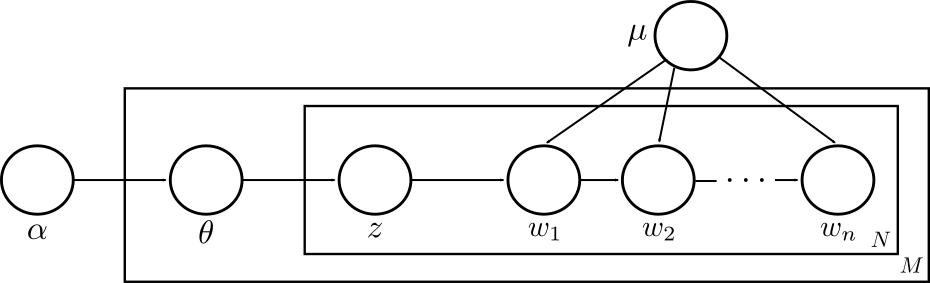
\includegraphics[width=\columnwidth]{./lda_mm_plate.pdf}
% \par\end{centering}
% \caption{Graphical Model for LDA with Markov Chain Topics\label{fig:lda-graphical-markov}}
% \end{figure}

A Markov Chain is a relatively compact way of specifying a distribution over strings of arbitrary length, requiring just $(|\Sigma| + 1)(|\Sigma| - 1)$ parameters (since each of the $|\Sigma| + 1$ multinomial distributions that make up a Markov Chain requires $|\Sigma| - 1$ parameters). The price paid for this representational efficiency is of course reduced expressivity; the space of string distributions that can be described via a Markov Chain is a small subset of the space of all possible string distributions.

\subsubsection{Hidden Markov Model Topics}

\subsubsection{Kalman Filter}

\subsubsection{Recurrent Neural Network}

\subsection{Relation to Latent Dirichlet Allocation}
TODO: Redo this section taking into account its new position.
We first briefly introduce Latent Dirichlet Allocation, which is the basis for our model. LDA was originally introduced as a means of inferring latent topics in a collection of documents. Each topic is a multinomial distribution over all possible words, and each document is taken to be a convex combination of the topics. Given a fixed set of parameters consisting of a concentration parameter $\alpha \in \mathbb{R}$ and a topic matrix $\beta \in \mathbb{R}^{K\times W}$ where the $k$-th row $\beta_{k, :}$ is a topic specifying a multinomial distribution over words, LDA assumes that the $i$-th document in the corpus is generated as follows. First, select topic mixture weights $\theta_i \sim \text{Dirichlet}(\alpha)$. Then for each word location $j \in [N]$, choose a topic for that location $z_{ij} \sim \text{Multinomial}(\theta_i)$, and generate a word the chosen topic $w_{ij} \sim \text{Multinomial}(\beta_{z_{ij}, :})$. The graphical model for this generative process is depicted in \fg~\ref{fig:lda-graphical}.

\begin{figure}[h!]
\begin{centering}
    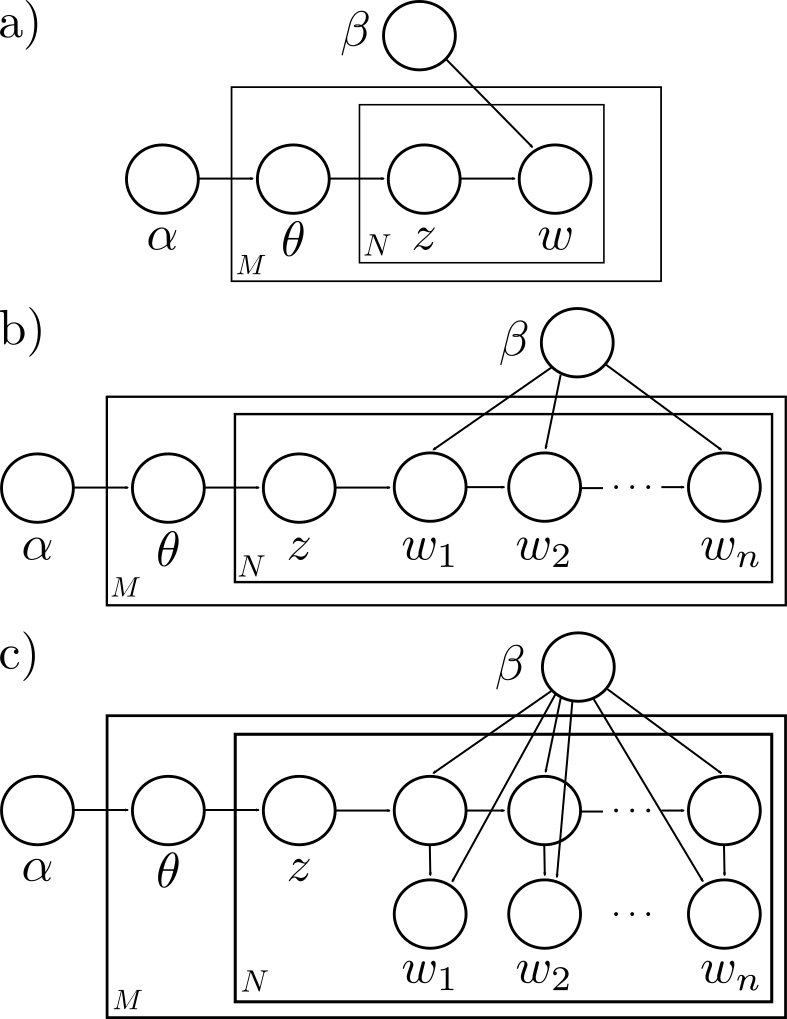
\includegraphics[width=\columnwidth]{./lda_plate_all.pdf}
\par\end{centering}
\caption{Graphical Models for a) LDA, b) LDA with Markov Topics, and c) LDA with HMM Topics.\label{fig:graphical-models}}
\end{figure}

During training, $\alpha$ and $\beta$ are unknown; we are given a corpus of $T$ documents and our goal is to learn $\alpha$ and $\beta$ for the corpus and $\theta_i$ for each document. This can be achieved by a number of algorithms; later in the paper we outline the original variational expectation-maximization algorithm. The learned model can then be used for \textit{document completion} where we predict other likely words in the documents we have already seen, \textit{document evaluation} where we evaulate the likelihood of previously unseen documents (the model should assign high likelihood to documents that are part of the corpus but were held out of the training data for testing purposes) and \textit{document classification}, where a document's distribution over topics $\theta_i$ is taken as a summary of the information contained therein and used as a description of the document for various classification tasks. As suggested by this last task, LDA has been called ``multinomial PCA'' by some authors, highlighting the fact that the topics a document contains can be taken to be a low-dimensional representation of the information that it contains.

The central insight of the current paper is that the LDA model can be used for multitask learning in many different learning settings by making an analogy between documents and tasks, and changing the family of distributions used as topics, replacing the multinomials used in vanilla LDA to another family that is more suitable for the application of interest. In the current work, we are interested in multitask \textit{sequence} learning, and consequently we take the topics to be sequence models (\eg markov chains and hidden markov models).

There are at least two benefits to making this switch: 1) it becomes possible to use the model for making predictions \textit{within} a word/sequence (\ie predicting the next character in a word/sequence) which is not readily possible when using a multinomial distribution over words/sequences, and 2) if the sequence generation model realizes a set of distributions over words that is smaller than the space of all possible distributions, then this can provide a form of regularization which may reduce the sample complexity of learning the model.

If one were alternatively interested in real-valued data, then the topic distributions could be Gaussians, and each document/task would consequently be modelled as a Gaussian mixture model, with each mixture component being shared by multiple documents/task.


\subsection{Prediction}

\section{Algorithm}
\subsection{Modelling Topics as Sequence Generators}

\section{Results}

\section{Discussion and Related Work}

\begin{tcolorbox}
\subsection{Notation}
\begin{itemize}
        \item $[n] = \{1, 2, \dots, n\}$ for $n \in \mathbb{N}$
        \item $\Delta^{k-1}$: the $k-1$ dimensional probability simplex. Contains all discrete distributions over $k$ options.
        \item $T$: number of documents/tasks
        \item $N$: number of words/sequences in each document
        \item $K$: number of topics
        \item $V$: number of unique words
        \item $\theta_i \in \Delta^{K-1}$: a discrete distribution over topics for the $i$-th document
        \item $\theta = \{\theta_1, \dots, \theta_M\}$
        \item $\beta_k \in \Delta^{V-1}$: a discrete distribution over words for the $k$-th topic
        \item $\beta = \{\beta_1, \dots, \beta_K\}$
        \item $z_{ij} \in [K]$: topic of the $j$-th token in the $i$-th document
        \item $Z_i = \{z_{i1}, \dots, z_{iN}\}$: topic variables for the $i$-th document
        \item $Z = \{Z_1, \dots, Z_M\}$: topic variables for the entire corpus
        \item $w_{ij} \in [V]$: word type of the $j$-th token in the $i$-th document
        \item $W_i = \{w_{i1}, \dots, w_{iN}\}$: word types for the $i$-th document
        \item $W = \{W_{1}, \dots, W_{M}\}$: word types for the entire corpus
        \item $\alpha \in \mathbb{R_+}$ or $\mathbb{R}^K_+$: parameter for the Dirichlet distribution over topic distributions
\end{itemize}
\end{tcolorbox}

\section{Learning Algorithm}
\subsection{Variational Expectation-Maximization for LDA}
In this section we review the original variational expectation-maximization algorithm for estimating LDA parameters $\alpha$ and $\beta$ and latent variables $\theta$ and $Z$. A number of improvements on this basic algorithm have been presented, including Gibbs Sampling, Collapsed Gibbs Sampling, etc., some of which could applied to our algorithm with minor modifications.

Assume we have been given a corpus of $T$ documents, call this $W$. Our goal is to learn values for parameters $\alpha$ and $\beta$ which maximize the log-likelihood of the observed corpus. The other unobserved variables, $Z$ and $\theta$, are treated as latent variables for which we will also obtain estimates. We can formulate the learning problem as one of maximizing the log-likelihood of the observed documents:
\begin{align}
    \max_{\alpha, \beta} \log P(W | \alpha, \beta)
\end{align}
Because of the latent variables $Z$ and $\theta$, this cannot be optimized directly. Instead, we derive a lower-bound on the log likelihood and maximize that. Let $Q$ be an arbitrary distribution over the latent variables. Then it can be shown that:
\begin{align}
    &\log P(W | \alpha, \beta)\\
    = &E_{Z, \theta \sim Q}\left[\log \frac{P(Z, \theta, W | \alpha, \beta)}{Q(Z, \theta)}\right] - \\
    &E_{Z, \theta \sim Q}\left[\log \frac{P(Z, \theta | \alpha, \beta)}{Q(Z, \theta)}\right]\\
    = &\mathcal{L}(\alpha, \beta, Q) + D_{KL}(Q(\cdot, \cdot) || P(\cdot, \cdot | \alpha, \beta))
\end{align}
Since the KL-divergence is non-negative, $\mathcal{L}(\alpha, \beta, Q)$ is a lower bound on the log-likelihood; thus it is often called a \textit{variational lower bound}. In EM, $\mathcal{L}$ is maximized by co-ordinate ascent. In particular, on the E-step $\mathcal{L}$ is maximized with respect to $Q$, while in the M-step $\mathcal{L}$ is maximized with respect to the parameters $\alpha$ and $\beta$.

\subsubsection{E-step}
To perform the E-step, we observe that $\log P(W | \alpha, \beta)$ does not depend on $Q$, so $\mathcal{L}$ is maximized with respect to $Q$ when the KL-divergence term is minimized, which is achieved when $Q(Z, \theta) = P(Z, \theta | W, \alpha, \beta)$. If $P(Z, \theta | W, \alpha, \beta)$ is tractable, then the E-step just consists of making this assignment. However, in case of LDA, $P(Z, \theta | W, \alpha, \beta)$ is not tractable. Instead, we perform a variational approximation; we select a tractable, parameterized family of distributions, and then perform free-form optimization with respect to those parameters to obtain the parameter setting that minimizes the KL-divergence term. This approximation is what makes it a \textit{variational} EM algorithm.

We select a family of distributions in which the $\theta_i \independent z_{i, j} \forall j \in [N]$ and $z_{ij} \independent z_{i\ell} \forall j \neq \ell$. That is, within a given document, we are explicitly ignoring dependencies both between the topic distribution $\theta_i$ and topic variables $z_{ik}$, and between pairs of topic variables. The distribution takes the form:
\begin{align}
    &Q(Z, \theta | \gamma, \phi)\\
    = &\prod_{i=1}^M Q(Z_i, \theta_i)\\
    = &\prod_{i=1}^M \left(Q(\theta_i | \gamma_i)\prod_{j=1}^N Q(z_{ij} | \phi_{ij})\right)
\end{align}
$\gamma_i \in \mathbb{R}^K_+$ is a set of variational parameters picking out a Dirichlet distribution for $\theta_i$. Likewise, $\phi_{ij} \in \Delta^{K-1}$ is a set of variational parameters picking out a Multinomial distribution for $z_{ij}$. The E-step then consists of solving the following optimization problem for the $i$-th document:
\begin{align}
    (\gamma^*_i, \phi^*_i) = \argmin_{\gamma_i, \phi_i} D_{KL}\left(Q(\cdot | \gamma_i, \phi_i) || P(\cdot | \alpha, \beta)\right)
\end{align}

\citet{blei2003latent} derive a co-ordinate descent algorithm for performing this optimization, whose updates take the form:
\begin{align}
    \phi_{ijk} &\propto \beta_{k, w_{ij}} \exp\{E_q[\log(\theta_{ik})]\}\\
    &= \beta_{k, w_{ij}} \exp\{\Psi(\gamma_{ik}) - \Psi(\sum_{\ell = 1}^K \gamma_{i\ell})\}\\
    \gamma_{ik} &= \alpha_k + \sum_{j=1}^N \phi_{ijk}
\end{align}
where $\Psi(\cdot)$ is the Digamma function. Each update corresponds to completely minimizing the KL-divergence w.r.t.\ one of the variables. For a single E-step, these updates are repeated until convergence.

\subsubsection{M-step}
Recall that the M-step consists of maximizing $\mathcal{L}(\alpha, \beta, Q)$ with respect to $\alpha$ and $\beta$. For $\beta$, the updates take the form:
\begin{align}
    \beta_{kw} \propto \sum_{i=1}^M \sum_{j=1}^N \phi_{ijk}\mathbbm{1}_{w_{ij} = w}
\end{align}
Basically, for each topic, the probability of each word is a normalized version of the sum of all the $\phi$ values for that topic-word combination. This comes from computing an M-projection of the distribution obtained by normalized the sum-of-phi's onto the space of multinomial distributions (i.e.\ the space of all discrete distributions; therefore no projection is really done at all). $L(\alpha, \beta, Q)$ is optimized w.r.t\ $\alpha$ using a fast Newton-Raphson method.

\begin{codebox}
\Procname{$\proc{E-Step}(W, \beta, \alpha)$}
\li\For$i \gets 1$ \To$M$
\li    \Do$\gamma^0_{ik} = \alpha_k+ N/K$ for all $j \in[K]$
\li    $\phi^0_{ijk} = 1/K$ for all $j \in[N], k \in[K]$
\li    $t \gets 0$
\li    \While\text{not converged}
\li        \Do\For$j \gets 1$ \To$N$
\li            \Do\For$k \gets 1$ \To$K$
\li                \Do$\phi^{(t+1)}_{ijk} \gets \beta_{k,w_{ij}} \exp\{\Psi(\gamma^{(t)}_{ik})\}$
                \End
\li            Normalize $\phi_{ij\cdot}$ to sum to 1
            \End
\li        \For$k \gets 1$ \To$K$
\li            \Do$\gamma^{(t+1)}_{ik} \gets \alpha_k+ \sum_{j=1}^N \phi^{(t+1)}_{jk}$
            \End
\li        $t \gets t + 1$
        \End
    \End
\li\Return$(\gamma, \phi)$
\end{codebox}

\begin{codebox}
\Procname{$\proc{M-Step}(W, \beta, \alpha)$}
\li\For$k \gets1$ \To$K$
\li     \Do \For $w \gets 1$ \To$M$
\li         \Do \For
        \End
    \End
\li\Return$(\gamma, \phi)$
\end{codebox}

\begin{codebox}
\Procname{$\proc{Latent-Dirichlet-Allocation}(W, \alpha, \beta)$}
\li$t \gets0$
\li\While\text{not converged}
\li    \Do$(\gamma, \phi) \gets \proc{E-Step}(W, \alpha, \beta)$
\li    $(\alpha, \beta) \gets \proc{M-Step}(W, \gamma, \phi)$
\li    $t \gets t + 1$
   \End
\end{codebox}

\subsection{Topics as Sequence Generators}
To modify the LDA learning algorithm to work with different families of topic-conditional distributions, we need only modify the M-step. For vanilla LDA, the M-step update described above arises from needing to solve the following optimization problem:
\begin{align}
    &\max_{\beta_{k,:}} \sum_{w=1}^V \left(\sum_{i=1}^M \sum_{j=1}^N \phi_{ijk}\mathbbm{1}_{w_{ij} = w}\right) \log P_{\beta_k}(w)\\
    = &\max_{\beta_{k,:}} \sum_{w=1}^V P_k(w) \log P_{\beta_k}(w)\label{eqn:dkl-mstep}
    %= &\min_{\beta_{k,:}} D_{KL}(P_k(\cdot) || P_{\beta_k}(\cdot))
\end{align}
where $P_{\beta_k}(w)$ is the probability of generating word $w$ from topic $k$ parameterized by $\beta_k$, and $P_k(w) \propto \sum_{i=1}^M \sum_{j=1}^N \phi_{ijk}\mathbbm{1}_{w_{ij} = w}$. Since we have been working with multinomial topics thus far, $P_{\beta_k}(w) = \beta_{kw}$, and the solution to \eqref{eqn:dkl-mstep} is $\beta_{kw} = P_k(w)$. The form of optimization given in \eqref{eqn:dkl-mstep} is even more useful, however, because it shows us how to perform the M-step for topic-conditional distributions other than the multinomial.

Some sequence models, such as $n$-th order Markov Models, provide a closed form solution to $\eqref{eqn:dkl-mstep}$. More expressive models that contain a notion of hidden state, such as Hidden Markov Models, can use Expectation-Maximization to obtain a local maximum of a lower bound of the objective. For other models, the objective can be maximized by stochastic gradient descent.

% \subsection{Time Complexity}
% \subsubsection{E-Step}
% All that changes on the E-step is how $\beta_{k,w}$ is computed. A naive implementation that computes $\beta$ by brute force would require an extra step for each E-step, the time complexity of which would be $O(K V \overline{|w|})$ where $\overline{|w|}$ is the average length  of words in the training set. However, it is likely that by storing the training words in a structure such as a suffix tree, the dependence on word-length can be significantly reduced. The algorithm would be something like: at the beginning of training, build a suffix tree from the training data. Then on each E-step, for each topic, create an annotated suffix tree where each edge is annotated by the probability that edge receives from the Markov Chain for that topic. Then traverse the suffix tree in order to fill in $\beta_k$. Should give a speedup, especially for datasets with small alphabets.
% 
% The complexity of the $E$-step in vanilla LDA is $O(MNKf(W))$, where $f(W)$ is the average number of iterations required for the variational optimization to converge. \citep{blei2003latent} found empirically that $f(W)$ tends to be on the order of $N$ (the number of words per document), yielding an approximate complexity of $O(MN^2K)$ per $E$-step.
% 
% \subsubsection{M-Step}
% We'll consider only maximizing $\mathcal{L}(\alpha, \mu, Q)$ w.r.t.\ $\mu$, since the maximization w.r.t.\ $\alpha$ is the same for our modified algorithm as it is for vanilla LDA. In vanilla LDA, solving for $\beta$ during the $M$-step requires $O(VK)$ runtime, since computing the sufficient statistics of $\phi$ and $\gamma$ which are necessary for the optimization can be folded into the E-step without changing its complexity. For our algorithm, the complexity of the $M$-step is $O(VK\overline{|W|_{trans}})$ where $\overline{|W|_{trans}}$ is the average number of unique transition types per word (e.g.\ if $\Sigma = \{0, 1\}$, then there are 4 possible transition types, but many words will have fewer than that. For example, $00000011111$ has only 3 transition types). The number of transition types in a word is always less than the length of the word, possibily signficantly so if the words are long and the alphabet is small.

% \begin{figure}[h!]
% \begin{centering}
%     \includegraphics[width=1.0\textwidth]{./markov_model_medium_likelihood_vs_n_train}
% \par\end{centering}
% \caption{3 topic, 10 characters, 100 words per doc \label{fig:results}}
% \end{figure}
% \begin{figure}[h!]
% \begin{centering}
%     \includegraphics[width=1.0\textwidth]{./markov_model_medium_likelihood_vs_n_topics}
% \par\end{centering}
% \caption{10 training docs, 10 characters, 100 words per doc \label{fig:results1}}
% \end{figure}


\bibliographystyle{apalike}
\bibliography{/home/eric/Dropbox/library}
\end{document}
